\documentclass[11pt]{article}

\usepackage[margin=1in]{geometry}
\usepackage{amsmath, amssymb}
\usepackage{graphicx}
\usepackage{hyperref}
\usepackage{booktabs}
\usepackage{enumitem}

\hypersetup{
    colorlinks=true,
    linkcolor=blue,
    citecolor=blue,
    urlcolor=blue
}

\title{
Residue Manifold Learning:\\
A Finite-State Model of Distributed Constraint Consistency, Projection, and Cost-Aware Stability
}

\author{
Dan Hawkley\\
\href{https://github.com/thinkthoughts/residue-manifold-learning}{github.com/thinkthoughts/residue-manifold-learning}
}

\date{May 2026}

\begin{document}

\maketitle

\begin{abstract}
We introduce a finite-state framework for analyzing distributed constraint consistency under noise. Using a modular residue manifold as a controlled setting, we show that local structural validity does not guarantee global coherence when systems are coupled by noisy links.

We define a distributed coherence metric (CGCS), demonstrate noise-driven degradation, and introduce projection as a constraint-preserving operator that restores consistency. A threshold condition characterizes when recovery succeeds, and a scaling law shows that maintaining global coherence becomes increasingly demanding with system size.

A phase diagram over link noise and projection success probability reveals distinct stability regimes. A spectral formulation connects the system to energy minimization, decoding, and constraint satisfaction. This provides a minimal model for distributed systems where interconnection quality governs global behavior.
\end{abstract}

\section{Introduction}

Distributed systems must maintain global consistency despite local noise and imperfect communication links.

While local structure may remain valid under noise, global coherence depends on consistency across connections. This distinction becomes dominant as systems scale.

Residue Manifold Learning (RML) provides a controlled finite-state setting to study this transition. Prior work established that:

\begin{itemize}[leftmargin=*]
\item modular residues define a discrete manifold,
\item sampling determines access to structure,
\item representation determines recovery versus fragmentation,
\item CGCS quantifies structural fidelity.
\end{itemize}

This perspective connects to prior work showing that structured sampling can collapse apparent quantum advantages into classical regimes \cite{tang2019}.

We extend this framework to distributed systems and study:

\begin{itemize}[leftmargin=*]
\item when local validity fails to ensure global consistency,
\item how link noise degrades coherence,
\item how projection restores valid constraints,
\item how stability scales with system size and noise.
\end{itemize}

Unlike traditional error-correction or constraint-satisfaction models, this framework isolates distributed consistency in a minimal finite-state setting.

\section{Residue Manifold}

\[
r = n \bmod 30
\]

Prime-support residues:
\[
R = \{1,7,11,13,17,19,23,29\}
\]

These form an eight-lane discrete manifold in $\mathbb{Z}/30\mathbb{Z}$.

\section{Constraint Graph Model}

We define a residue constraint graph:
\[
G = (V, E, R, D)
\]

\begin{itemize}[leftmargin=*]
\item $V$: nodes with residues $r \in R$
\item $E$: edges enforcing pairwise constraints
\item $D = \{(a-b)\bmod 30 : a,b \in R\}$
\end{itemize}

Constraint condition:
\[
(r_i - r_j) \bmod 30 \in D
\]

This defines a finite-state constraint system over residue assignments.

\section{Distributed Consistency Under Noise}

Nodes preserve local structure, while edges enforce global consistency. Thus consistency is a property of edges, not nodes.

\begin{figure}[htbp]
\centering
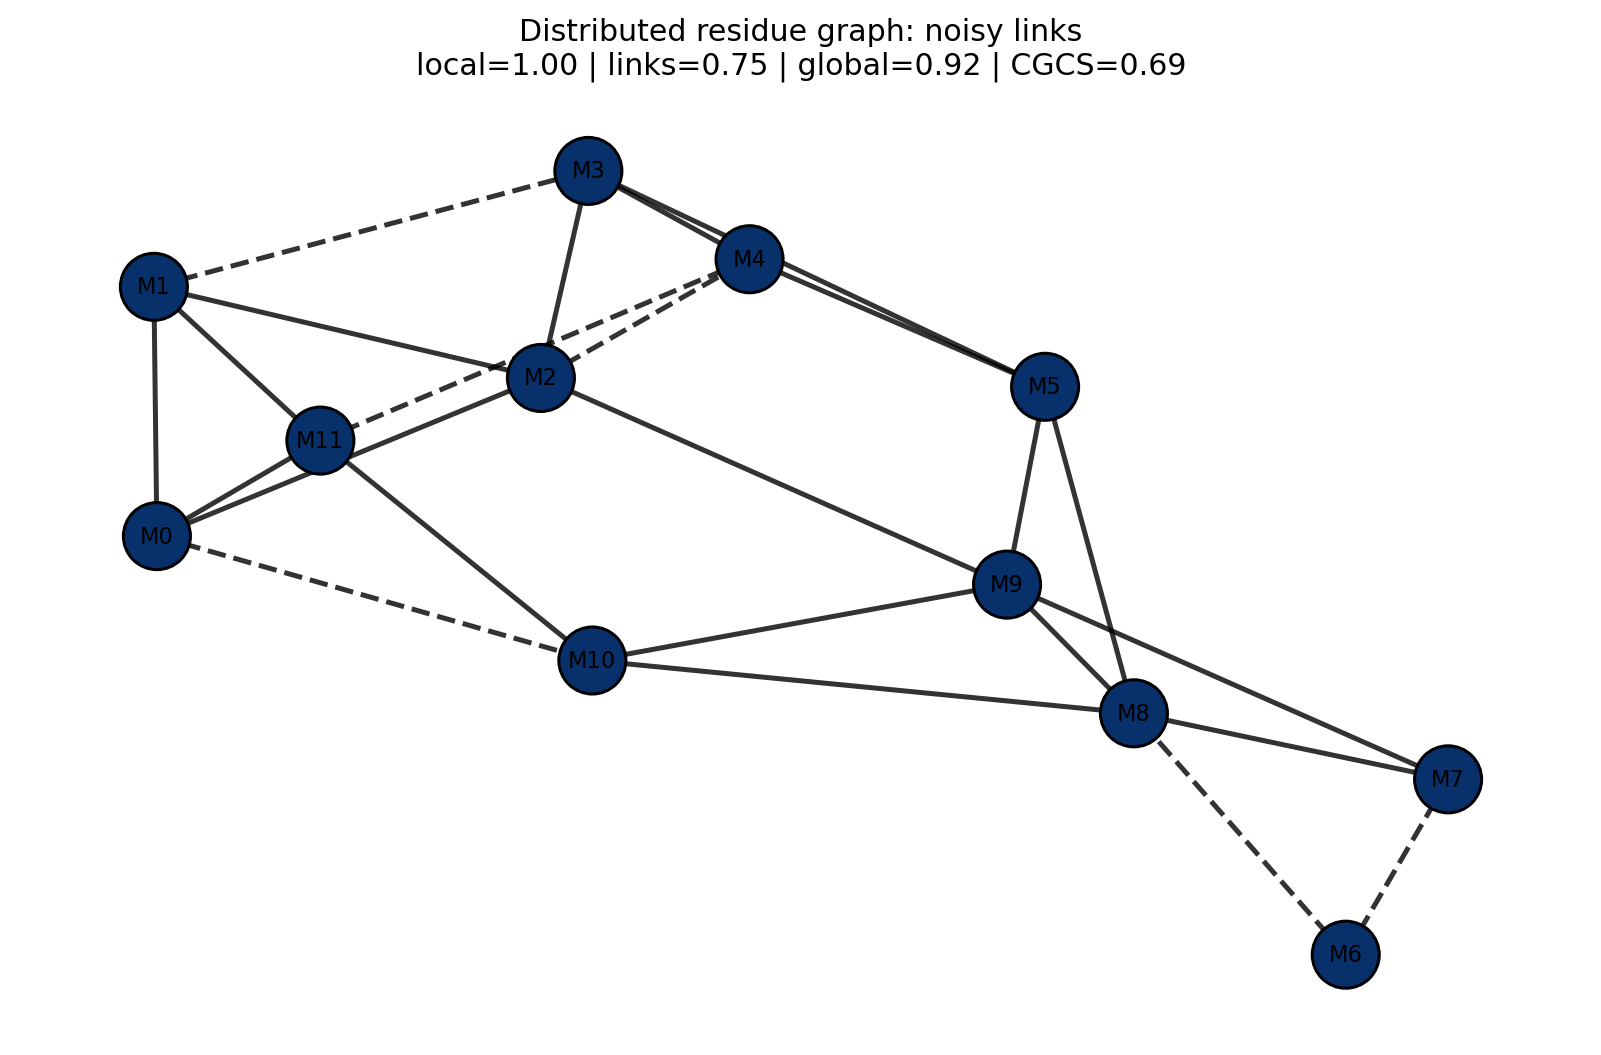
\includegraphics[width=0.8\linewidth]{figures/distributed_residue_graph_noisy.png}
\caption{Distributed residue graph under noisy links. Nodes remain locally valid while edges violate constraints.}
\end{figure}

\section{Constraint-Guided Coherence Score}

We use:

\begin{itemize}[leftmargin=*]
\item $\mathrm{CGCS}_{dist}$: distributed coherence score
\item $\mathrm{CGCS}_{eff}$: cost-adjusted coherence score
\end{itemize}

\[
\mathrm{CGCS}_{dist} =
(\text{local coverage})
(\text{local validity})
(\text{link consistency})
(\text{global stability})
\]

Threshold:
\[
\mathrm{CGCS} \ge \frac{24}{25}
\]

\section{Noise-Driven Degradation}

\begin{figure}[htbp]
\centering
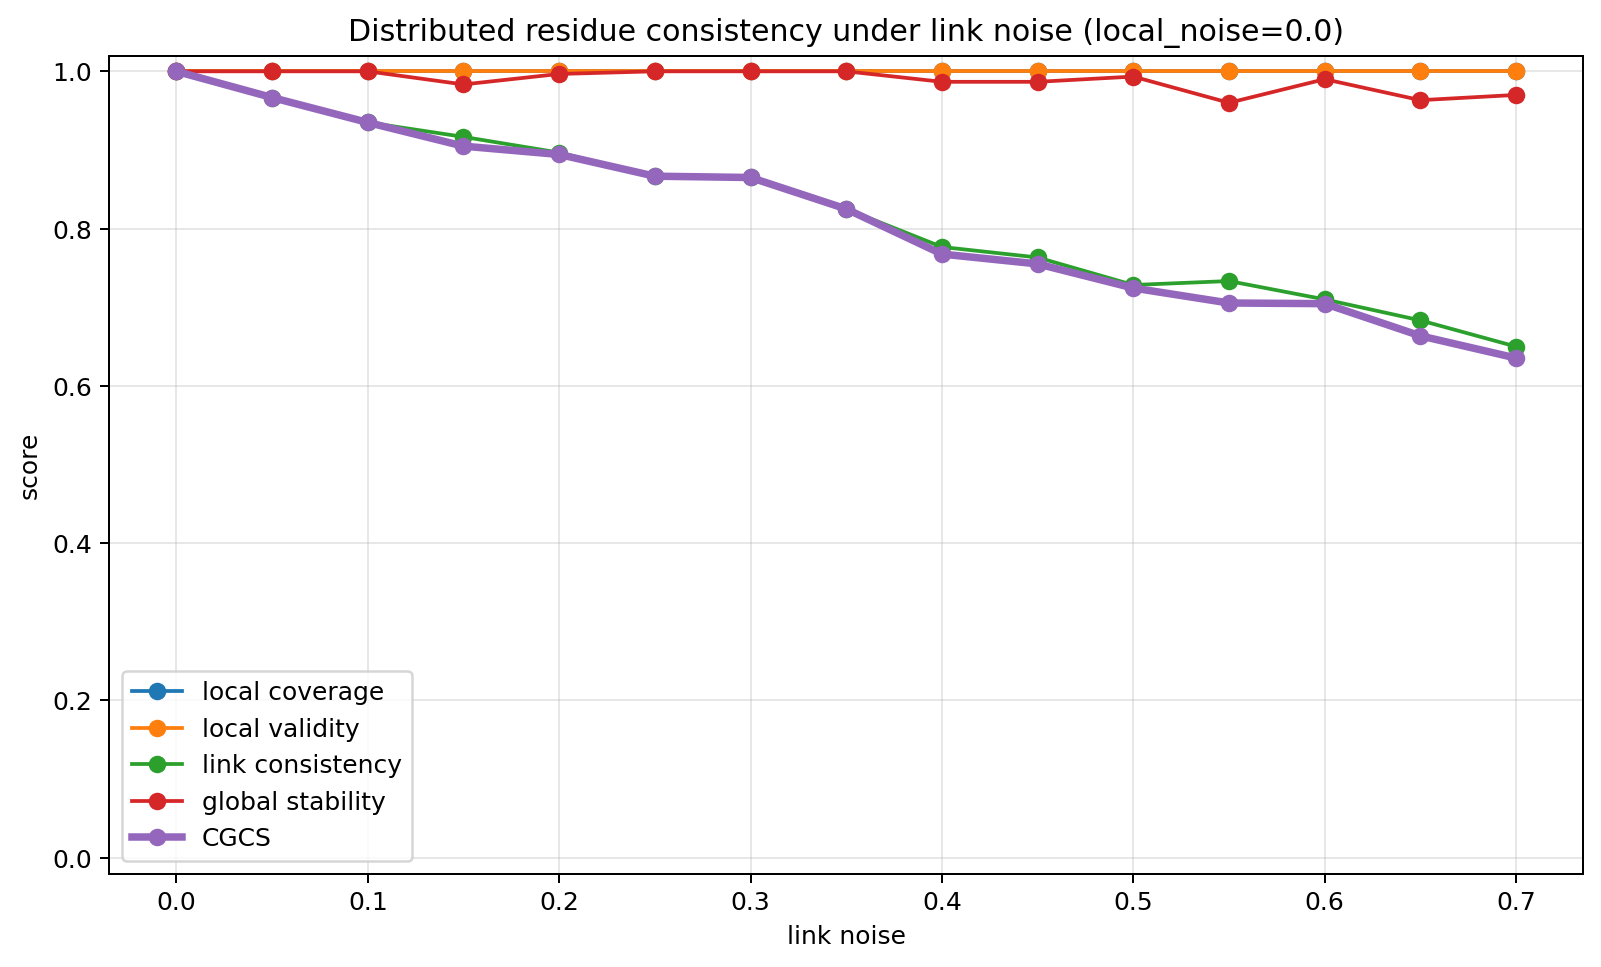
\includegraphics[width=0.8\linewidth]{figures/cgcs_noise_sweep.png}
\caption{Local validity remains high while link consistency degrades with increasing link noise, demonstrating that global coherence depends on inter-node constraints.}
\end{figure}

\begin{figure}[htbp]
\centering
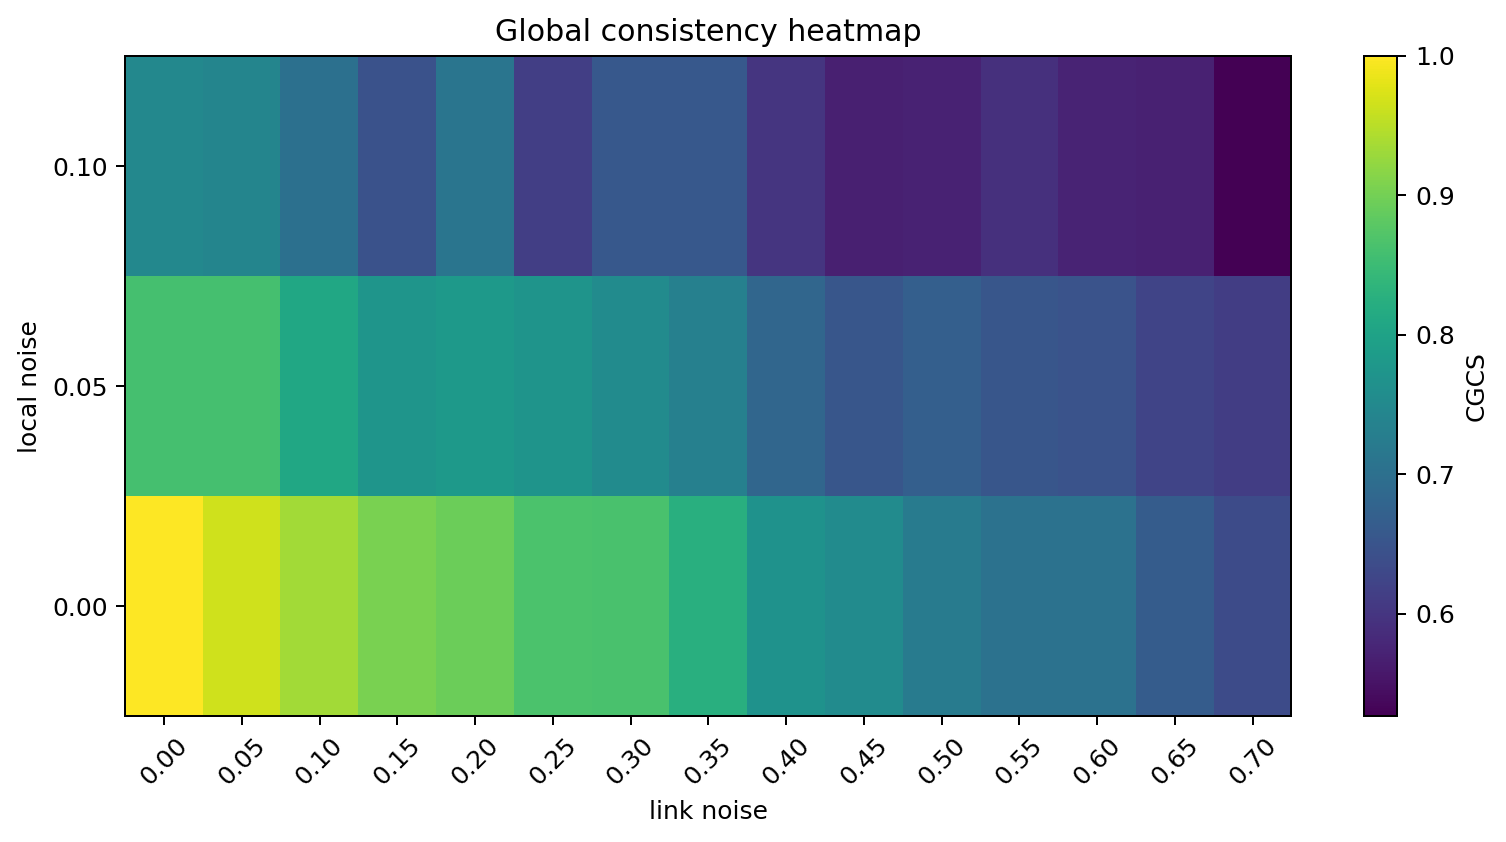
\includegraphics[width=0.8\linewidth]{figures/global_consistency_heatmap.png}
\caption{Global consistency as a function of local and link noise. Link noise dominates degradation.}
\end{figure}

\section{Projection as Constraint Operator}

Projection enforces constraint consistency by mapping:
\[
P : \mathbb{Z}/30\mathbb{Z} \rightarrow D
\]

\[
P(d_{obs}) = \arg\min_{d \in D} \mathrm{dist}_{30}(d_{obs}, d)
\]

\[
\text{noisy relation} \rightarrow \text{valid constraint}
\]

\begin{figure}[htbp]
\centering
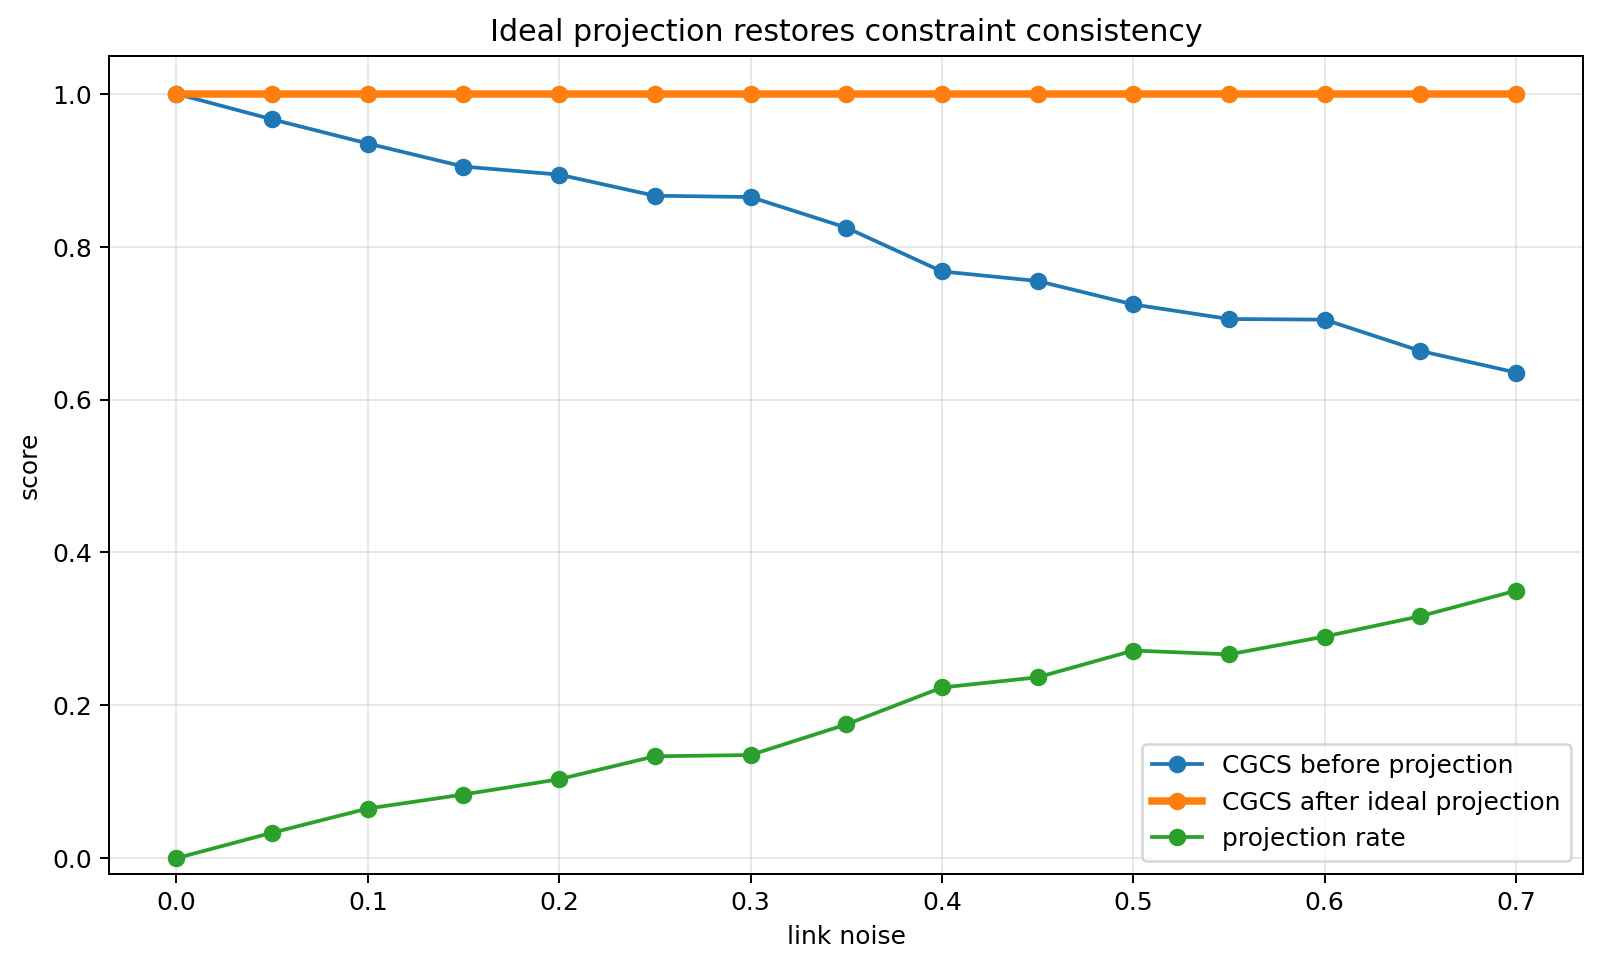
\includegraphics[width=0.8\linewidth]{figures/cgcs_projection_sweep.png}
\caption{Projection restores constraint consistency by mapping noisy relations to the nearest admissible constraint, recovering global coherence.}
\end{figure}

\section{Projection Thresholds}

Let:
\begin{itemize}[leftmargin=*]
\item $\rho$ = fraction of inconsistent links
\item $p_{success}$ = projection success probability
\end{itemize}

Consistency requires:
\[
p_{success} \cdot \rho \ge \rho_{\mathrm{crit}}
\]

Below threshold:
\[
\text{global consistency collapses}
\]

This defines a transition between stable and unstable regimes.

\section{Scaling Law}

Assuming independent link noise:

\[
|E| \sim 
\begin{cases}
O(N) & \text{sparse} \\
O(N^2) & \text{dense}
\end{cases}
\]

\[
\rho(N) \sim 1 - (1 - p_{noise})^{|E|}
\]

\[
p_{success} \ge \frac{\rho_{\mathrm{crit}}}{\rho(N)}
\]

Larger systems require stronger projection performance.

\section{Cost-Aware Stability}

\[
\mathrm{CGCS}_{eff} =
\mathrm{CGCS}_{after}(1 - \alpha \cdot \text{projection rate})
\]

\begin{figure}[htbp]
\centering
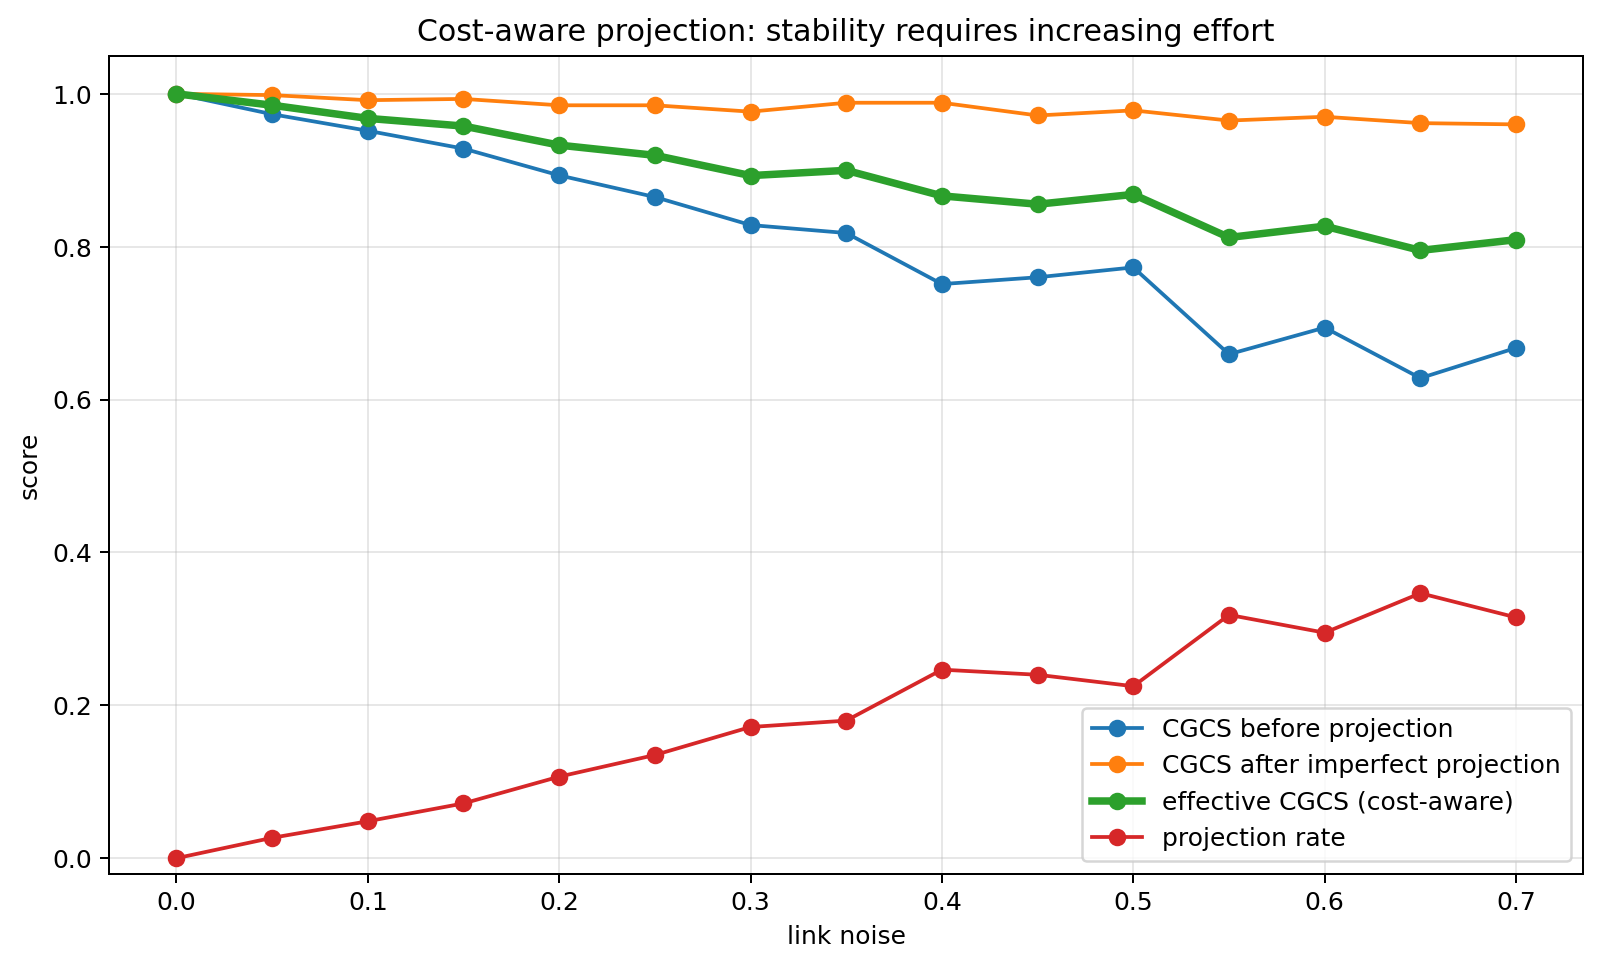
\includegraphics[width=0.8\linewidth]{figures/cgcs_cost_aware_projection.png}
\caption{Effective coherence decreases as correction effort increases, showing that stability is limited by available projection resources.}
\end{figure}

\section{Phase Structure}

We summarize the empirical phase structure as follows:

\begin{figure}[htbp]
\centering
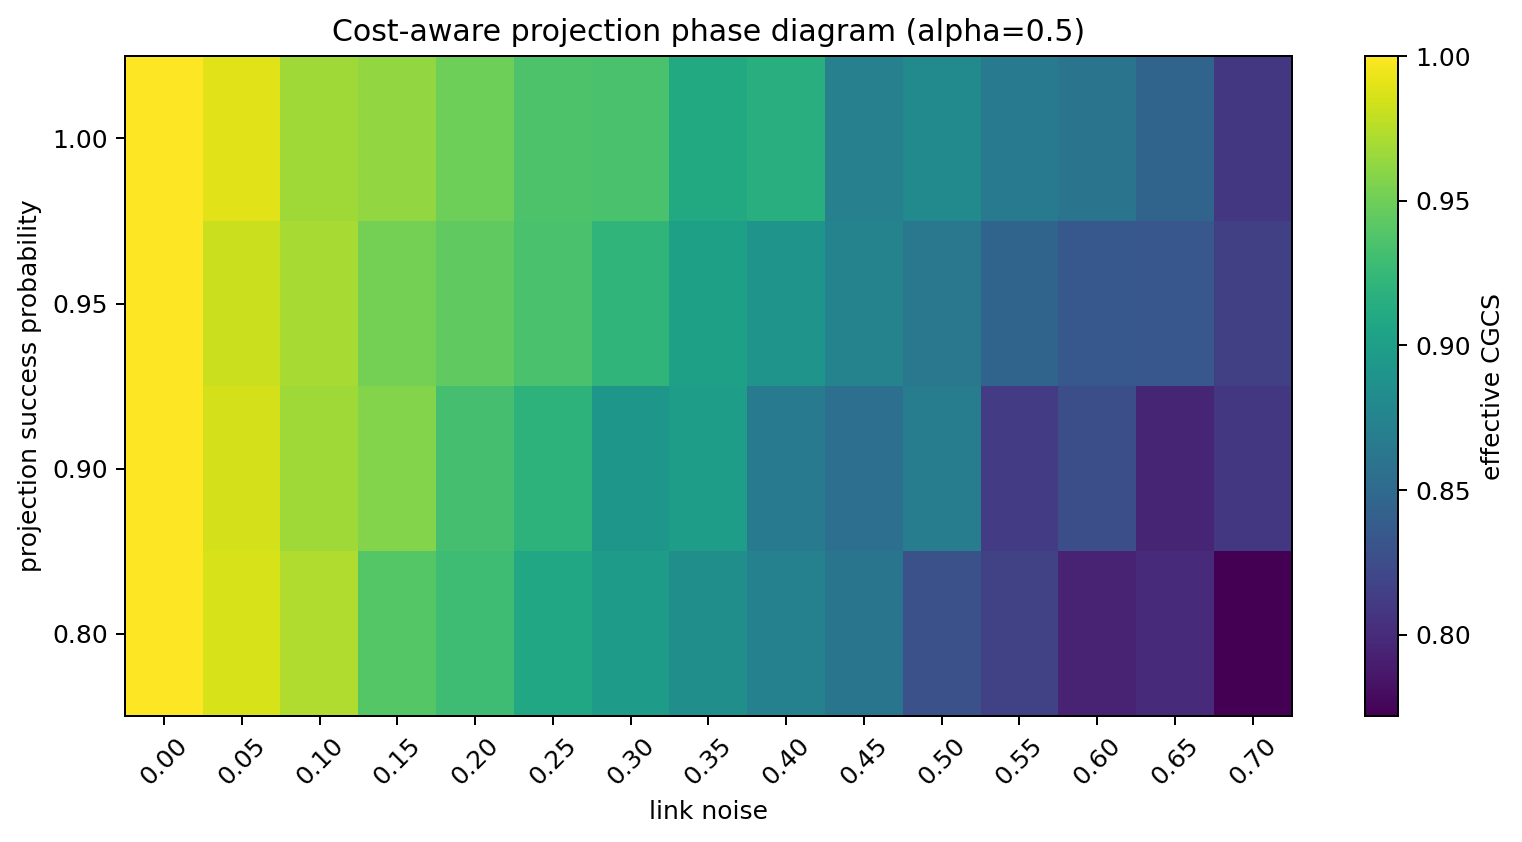
\includegraphics[width=0.8\linewidth]{figures/cost_aware_projection_phase_diagram.png}
\caption{Phase diagram over link noise and projection success probability. Stable, cost-limited, and degraded regimes emerge, with a threshold separating recoverable and unrecoverable consistency.}
\end{figure}

\section{Spectral Consistency}

This formulation makes the connection to classical constraint satisfaction explicit \cite{koller2009}.

\[
E(G) = \sum_{(i,j)\in E} \mathrm{dist}_{30}(r_i - r_j, D)^2
\]

\[
\mathrm{CGCS} \approx 1 - \frac{E(G)}{E_{max}}
\]

Projection:
\[
P(r) = \arg\min E(G)
\]

Interpretation:

\begin{itemize}[leftmargin=*]
\item noise injects constraint energy
\item projection minimizes energy
\item consistency corresponds to low-energy states
\end{itemize}

\section{Connection to Distributed Quantum Systems}

Projection plays a role analogous to decoding in quantum error correction, where noisy syndromes are mapped back to valid logical states \cite{gottesman2010}.

\begin{center}
\begin{tabular}{ll}
\toprule
RML & Distributed FTQC \\
\midrule
Residue states & Logical states \\
Link noise & Interconnect errors \\
Projection & Decoding \\
CGCS & Stability metric \\
\bottomrule
\end{tabular}
\end{center}

\section{Conclusion}

We show:

\begin{itemize}[leftmargin=*]
\item local correctness is insufficient for global coherence,
\item link noise dominates scaling behavior,
\item projection restores constraint validity,
\item stability requires increasing correction effort.
\end{itemize}

This provides a minimal model of distributed systems where interconnection quality determines global behavior.

\bibliographystyle{plain}
\bibliography{references}

\end{document}
